\begin{figure}[!h]
    \centering
	\begin{subfigure}[t]{\textwidth}
	    \centering
		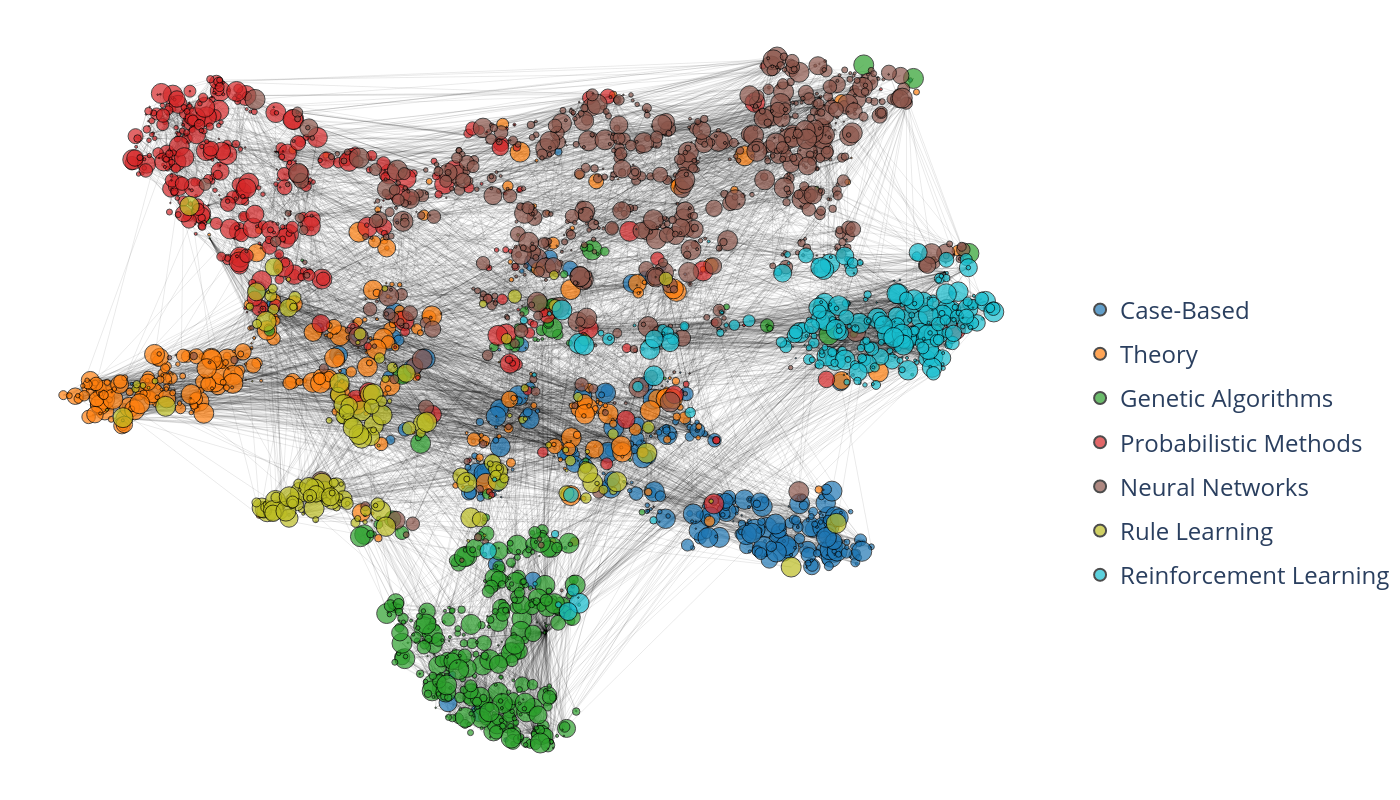
\includegraphics[height=0.25\textheight]{sections/009_neurips2021/resources/clean-classes.png}
		\caption{Ground-Truth Classes} 
		\label{subfig:latent-clean-classes}
	\end{subfigure}
	\begin{subfigure}[t]{\textwidth}
	    \centering
		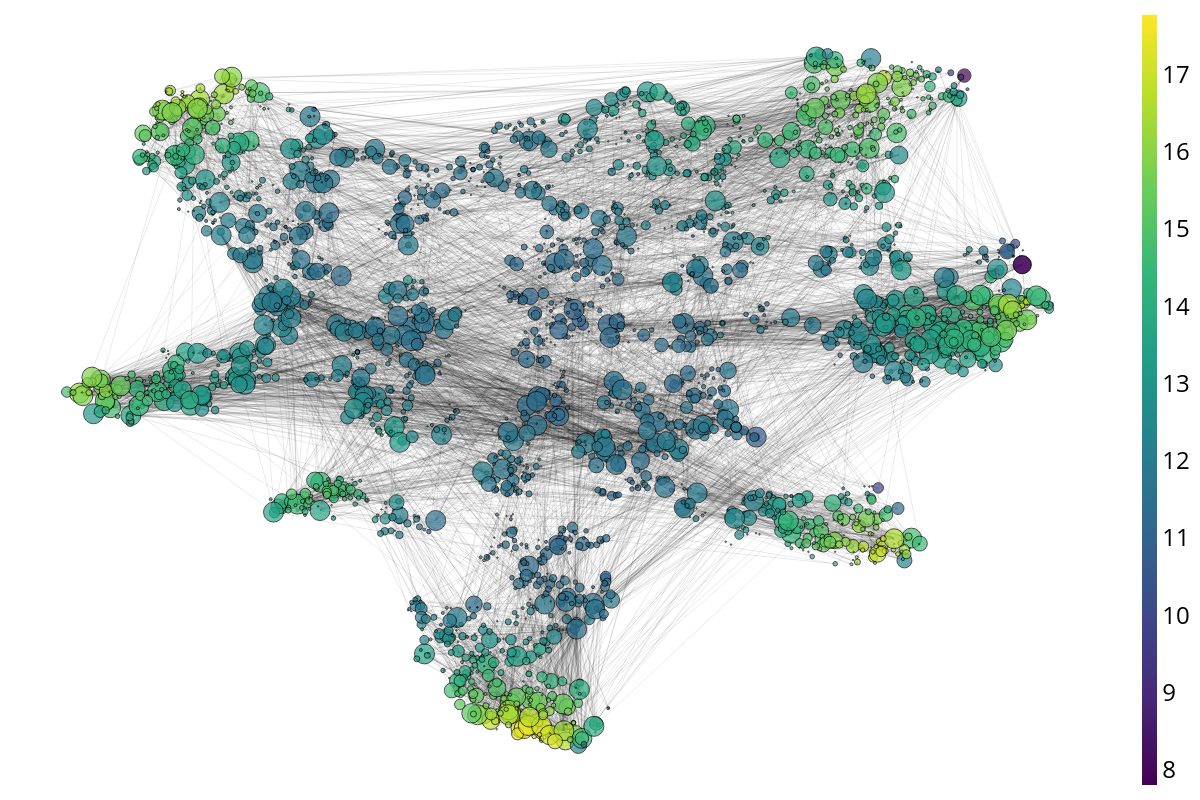
\includegraphics[height=0.25\textheight]{sections/009_neurips2021/resources/clean-ft-evidence.png}
		\caption{Feature Evidence} 
		\label{subfig:latent-clean-feature-evidence}
	\end{subfigure}
	\begin{subfigure}[t]{\textwidth}
	    \centering
		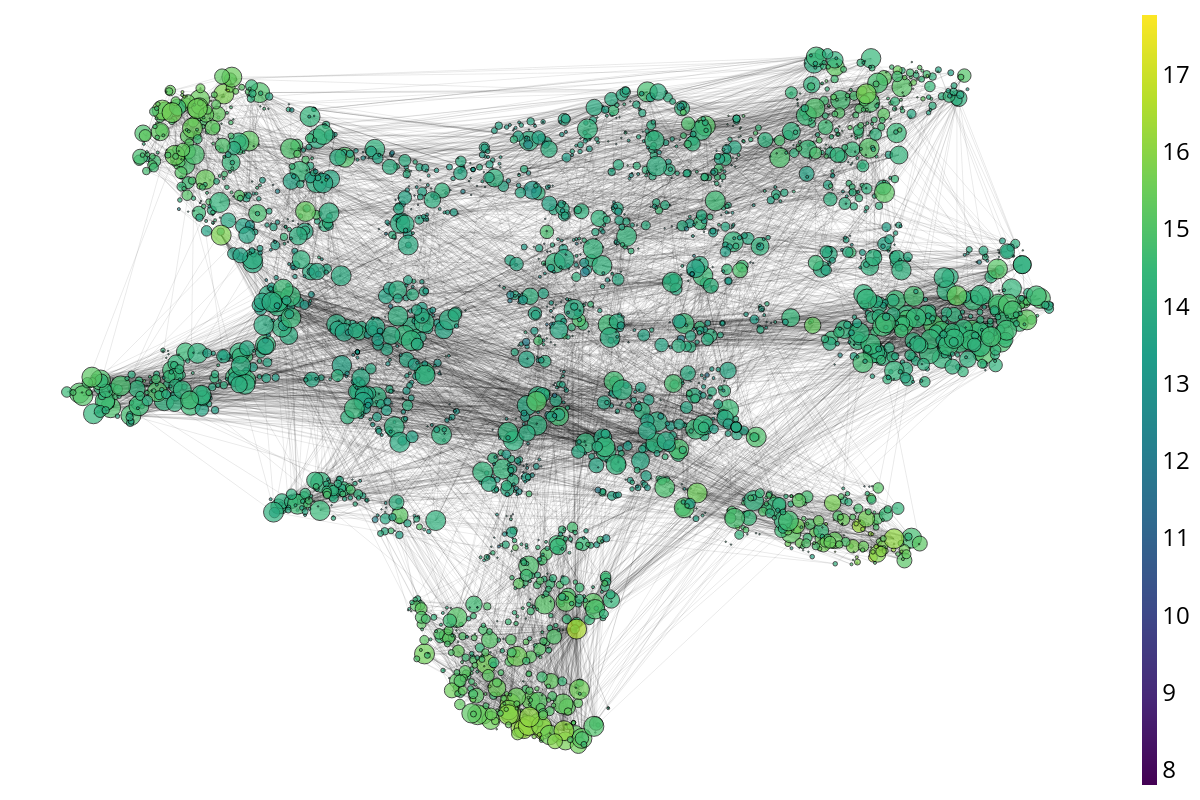
\includegraphics[height=0.25\textheight]{sections/009_neurips2021/resources/clean-evidence.png}
		\caption{Aggregated Evidence}
		\label{subfig:latent-clean-evidence}
	\end{subfigure}
    \caption{Latent space visualizations on the clean CoraML graph. The ground-truth classes are shown in different colors. The feature and aggregated evidence are represented in log-scale.}
    \label{fig:latent-space-clean}
\end{figure}
%
\begin{figure}[!h]
    \centering
	\begin{subfigure}[t]{\textwidth}
	    \centering
		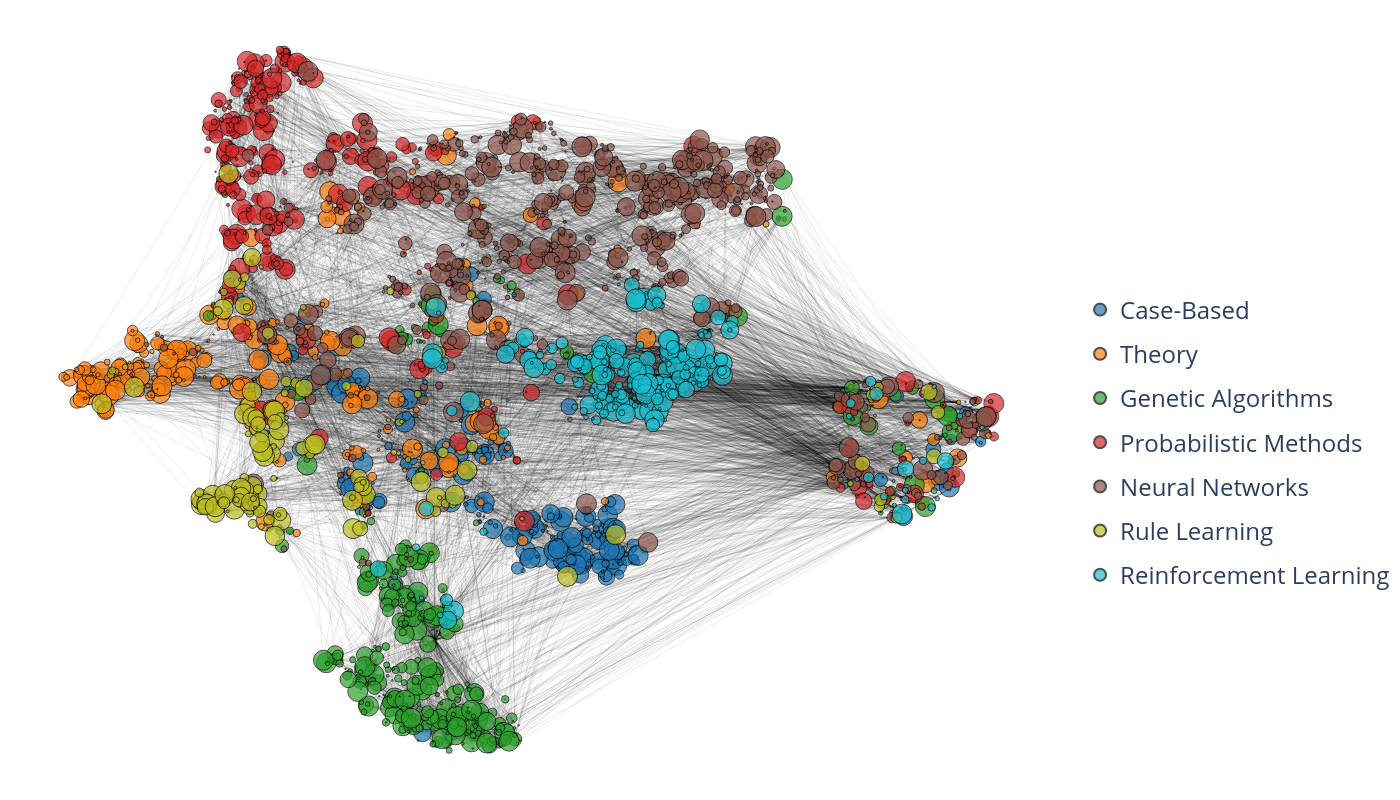
\includegraphics[height=0.25\textheight]{sections/009_neurips2021/resources/gaussian-classes.png}
		\caption{Ground-Truth Classes} 
		\label{subfig:gaussian-clean-classes}
	\end{subfigure}
	\begin{subfigure}[t]{\textwidth}
	    \centering
		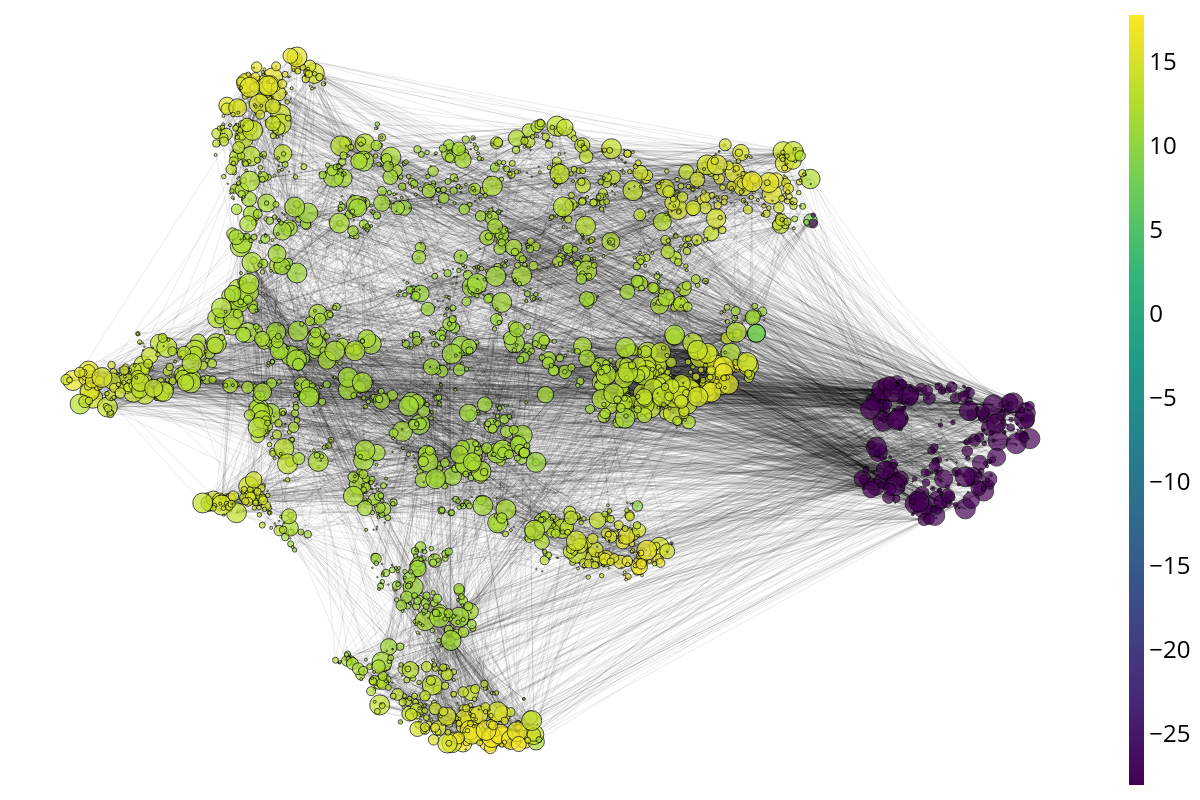
\includegraphics[height=0.25\textheight]{sections/009_neurips2021/resources/gaussian-ft-evidence.png}
		\caption{Feature Evidence} 
		\label{subfig:gaussian-clean-feature-evidence}
	\end{subfigure}
	\begin{subfigure}[t]{\textwidth}
	    \centering
		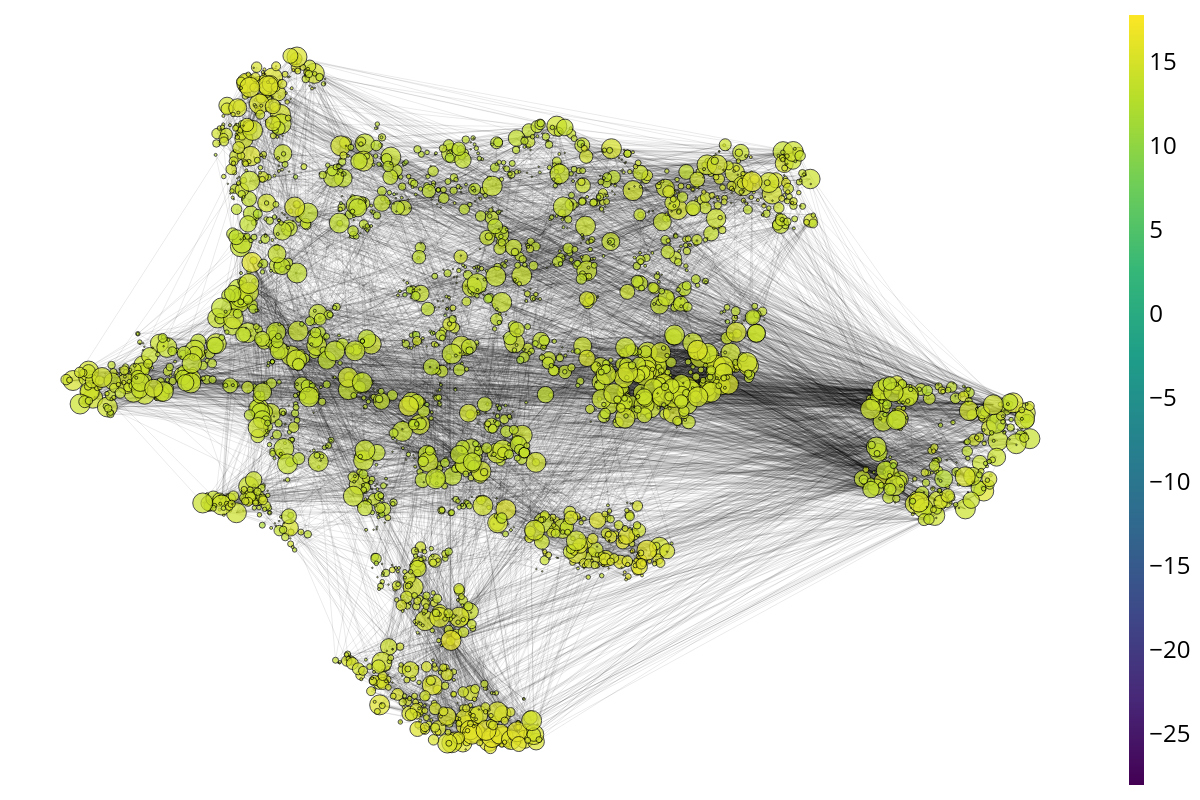
\includegraphics[height=0.25\textheight]{sections/009_neurips2021/resources/gaussian-evidence.png}
		\caption{Aggregated Evidence}
		\label{subfig:gaussian-clean-evidence}
	\end{subfigure}
    \caption{Latent space visualizations on the CoraML where $10\%$ of the nodes are perturbed with unit Gaussians. The ground-truth classes are shown in different colors. The feature and aggregated evidence are represented in log-scale.}
    \label{fig:latent-space-gaussian}
\end{figure}
%
\begin{figure}[!h]
    \centering
	\begin{subfigure}[t]{\textwidth}
	    \centering
		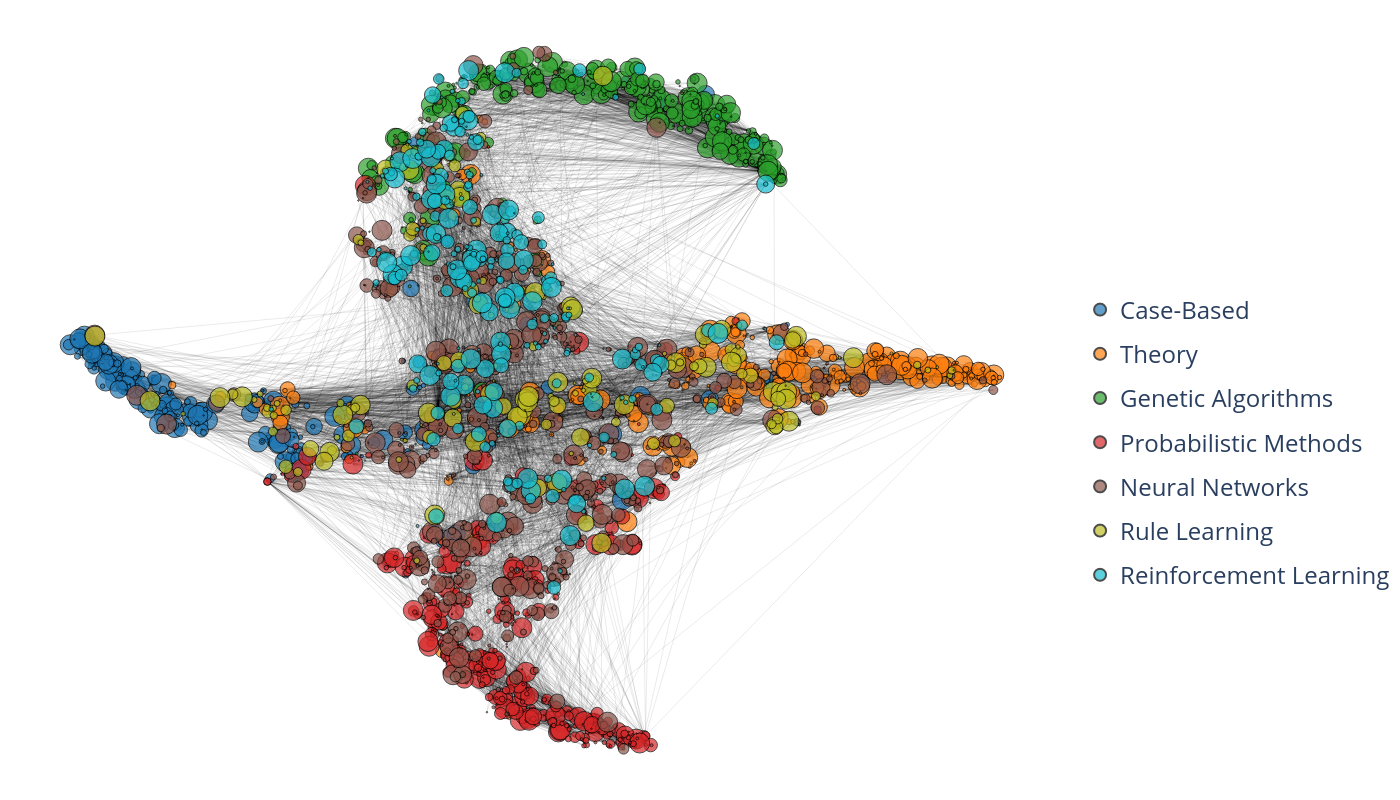
\includegraphics[height=0.25\textheight]{sections/009_neurips2021/resources/loc-classes.png}
		\caption{Ground-Truth Classes} 
		\label{subfig:loc-clean-classes}
	\end{subfigure}
	\begin{subfigure}[t]{\textwidth}
	    \centering
		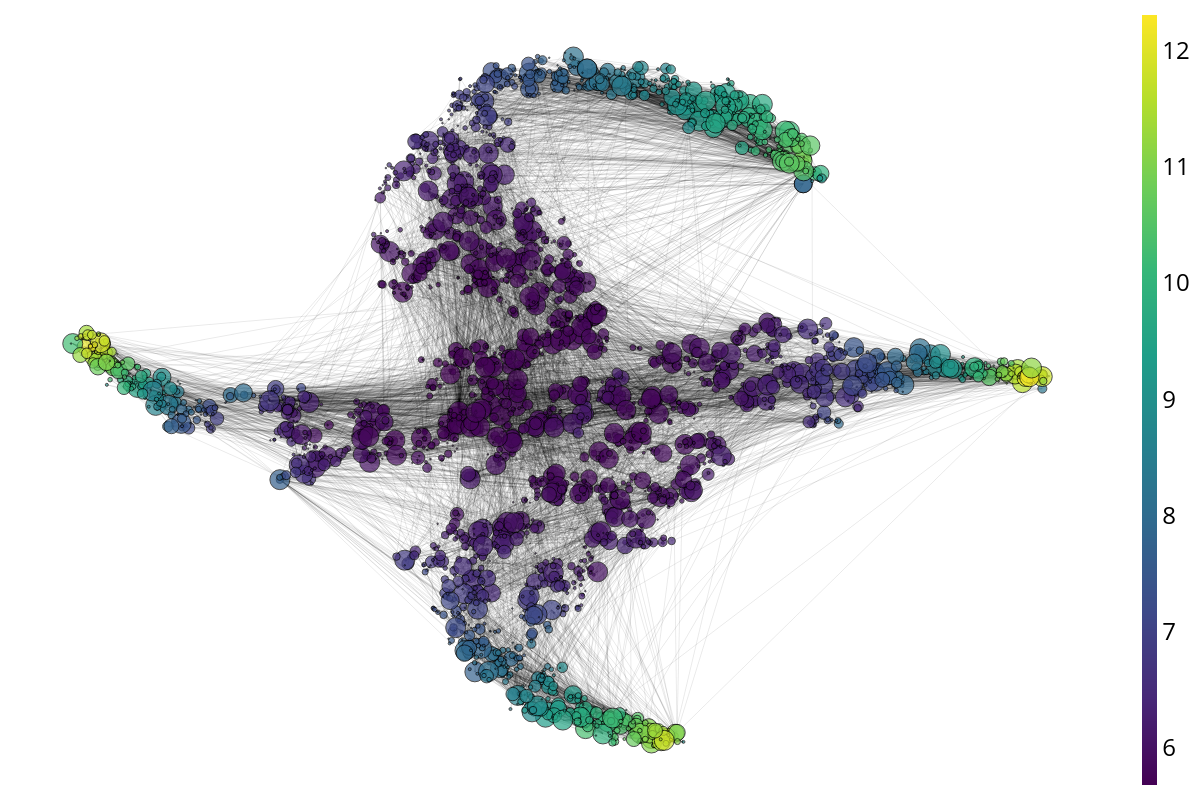
\includegraphics[height=0.25\textheight]{sections/009_neurips2021/resources/loc-ft-evidence.png}
		\caption{Feature Evidence} 
		\label{subfig:loc-clean-feature-evidence}
	\end{subfigure}
	\begin{subfigure}[t]{\textwidth}
	    \centering
		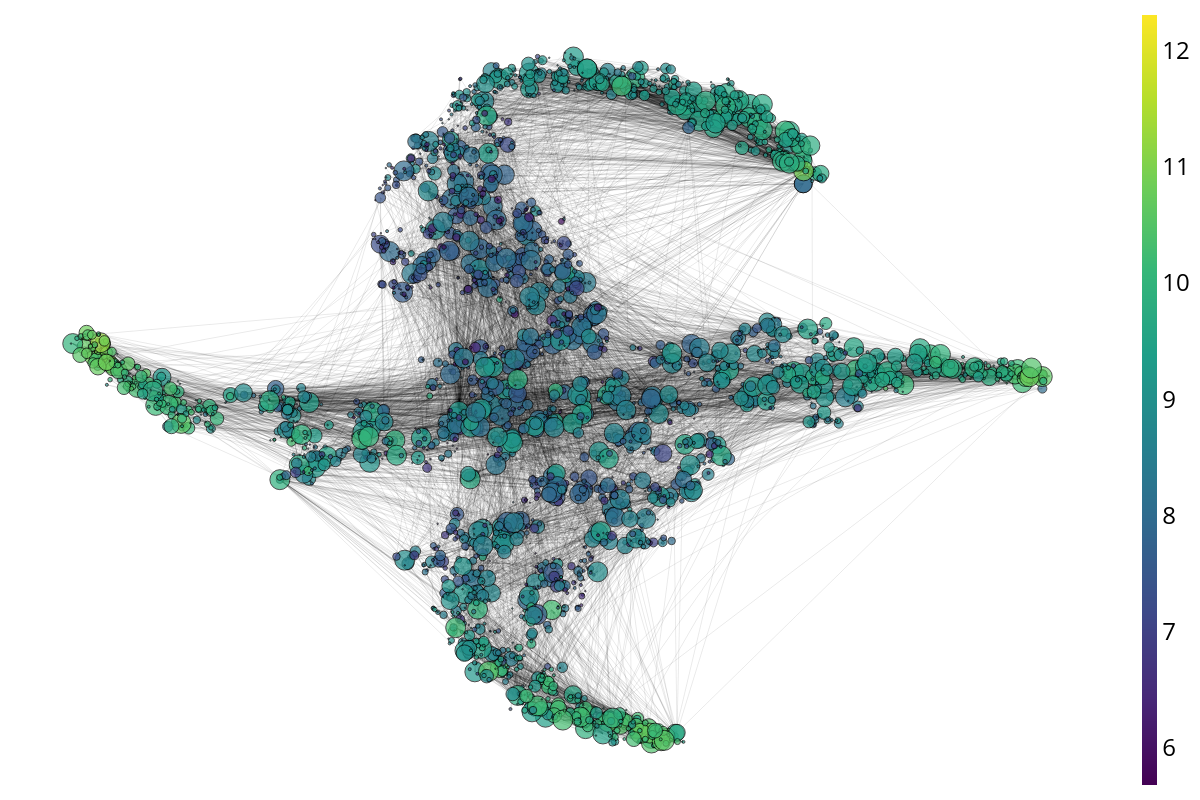
\includegraphics[height=0.25\textheight]{sections/009_neurips2021/resources/loc-evidence.png}
		\caption{Aggregated Evidence}
		\label{subfig:loc-clean-evidence}
	\end{subfigure}
    \caption{Latent space visualizations on the CoraML with Left-Out classes experiments. The ground-truth classes are shown in different colors. Nodes of the classes \emph{Neural Networks}, \emph{Rule Learning}, and \emph{Reinforcement Learning} have been left out for training but are kept in the graph. The feature and aggregated evidence are represented in log-scale.}
    \label{fig:loc-space-gaussian}
\end{figure}